\section{Approach}
\label{sec:approach}
%Opinion summarization aims at generating abstractive 
%summaries covering salient opinions expressed in multi-reviews.
We denote $\mathbb{R}=(R^1, ..., R^E)$ as the review corpus with $E$ entities. % (e.g. products or restaurants). 
$R^e$ contains all of the reviews of entity $e$. %in the whole dataset.
As $\mathbb{R}$ has no reference summaries for training,
we designed a weakly supervised approach and an
aspect-guided model as follows.
%by first
%constructing a semi-structured training set 
%with opinion-aspect pairs (OAs) and implicit sentences (ISs) as input, and then 
%\KZ{$R^e$ is a multi-review about entity $e$? Then why you have the overline thingy later?}
%Since there is no human-annotated data for training, our approach is weak supervised.


\subsection{Semi-structured Training Data Creation}
\label{sec:data}
To avoid information loss in textual inputs or structured inputs,
% (as shown in \figref{fig:brief}),
we create a synthetic semi-structured training dataset $\mathbb{D}$ with four steps, 
%by first sampling textual outputs, i.e. summaries, and then sampling semi-structured inputs, including noisy OAs and noisy ISs corresponding to each output. %The  intuition behind noising operations is to simulate the summarization process for real multi-reviews. \KZ{Don't repeat things
%you have said in the intro or previously.}
%sampling semi-structured inputs, including opinion-aspect pairs (OAs) and implicit sentences (ISs), and textual summary outputs. 
%IS is the sentence that we cannot extract OAs from, which can be regarded as the supplymentary of OAs.
%Our method consists of four parts, 
as shown in \figref{fig:dm}: 
%(1) we extract OAs and ISs from $R_e$%the reviews of entity $e$,
%(2) we sample a review as a summary $y$, 
%(3) {\em opinion-aspect pairs noising} selects proper OAs from $P^e$ to get noisy OAs for $y$,
%and (4) {\em implicit sentences noising} selects noisy sentences from $S^e$ 
%that different from ISs in $y$.
(1) \textbf{sampling a review} as a summary $y$ from all reviews $R^e$ of an entity $e$ and the others are candidate reviews $\overline{R^e}$; 
(2) \textbf{extracting OAs and ISs} from $\overline{R^e}$ to 
obtain the OA's group $\overline{P^e}$
and IS's group $\overline{S^e}$;
(3) {\bf opinion-aspect pairs noising} samples proper OAs from $\overline{P^e}$ to 
obtain {noisy OAs for $y$;
and (4) {\bf implicit sentences noising} samples noisy ISs from $\overline{S^e}$. 
%\JQ{I exchanged (1) and (2)}
%The OAs an ISs in real multi-review can be seen as the noisy version of them in reference summary, 
%Taking noisy OAs and ISs as input simulates the process of summarization for OAs and ISs of multi-reivew.
% during generation. 
%The process is shown in \figref{fig:dm}.
\begin{figure}[th]
	\centering
	\includegraphics[width=0.9\linewidth]{./dm.pdf}
	\caption{Semi-structured training data creation.}
	\label{fig:dm}
\end{figure}

\cut{%%%
We use $R^e=(r_1,...,r_M)$ to denote all reviews of an entity $e$. 
For a review $r$, 
we extract opinion-aspect pairs, 
$p=(p_{1},...,p_{d})$, 
expressing opinions of the reviewer towards aspects of the entity.
$p_i$ denotes the set of OAs for the $i$-th aspect.
$p_{i}=\{(o_{1,i}, f_1), ..., (o_{n,i}, f_n)\}$ where %$o_{j,i}=(o_j, a_i)$. 
$o_{j,i}$ is $j$-th OA pair of aspect $a_i$ 
and $f_j$ is the number of occurrences of $o_{j,i}$.
We use $s=(s_1,..., s_k)$ to denote the  ISs in review $r$. % ISs usually express the implicit opinion of the entity.
Thus, the review $r$ is represented by a set of OAs and a set of ISs.
The OAs of $R_e$ compose an OA group $P^e=(P_{1},...,P_{D})$, 
where $P_{i}=\{(o_{1,i},f_1), ..., (o_{N, i},f_N)\}$ and $D$ represents the number of aspects.
The ISs of $R_e$ compose an IS group $S^e=(s_1,..., s_K)$. 
}%%%%



\textbf{Summary Sampling.} 
%Wefollow~\citet{Denoise20} with sampling 
We take a sampled review of entity $e$ as {\em summary} ($y$) and the other reviews of $e$ as {\em candidate reviews} ($\overline{R^e}$).
%Similarly, 
We ignore the reviews containing first-person singular pronouns
and non-alphanumeric symbols except punctuation~\cite{Denoise20},
because such reviews are not similar to real summaries. %\KZ{Why?}
Besides, we ensure that all aspects of the summary can be found in $\overline{R^e}$.
This stems from the fact that aspects in the summary should not come  
from outside of its multi-review.

\textbf{Opinion-aspect Pairs and Implicit Sentences Extraction.} 
%For every review, we utilize a rule-based MIN-MINER~\cite{basicOpiMin20} to get the dependency parse trees of sentences first and then use a set of syntactic rules~\cite{aspect12} to extract OAs.
\cut{%%%%
We obtain OAs for every review in corpus by a rule-based
MIN-MINER~\cite{basicOpiMin20} . 
It gets the dependency
parse trees of sentences first and then uses a set of syntactic rules~\cite{aspect12} to extract opinion-aspect pairs.
~\footnote{It is flexible to use different opinion-aspect extractions.}
}%%%%
%We follow \citet{Denoise20} with sampling a review from the corpus as summary.
%The summary must be no first-person singular pronouns, 
%and no non-alphanumeric symbols aside from punctuation.
%We sample a review of entity $e$ as {\em summary},
%The review can be represented by OAs and ISs.
We utilize a rule-based MIN-MINER~\cite{basicOpiMin20} to get the dependency parse trees of sentences first and then use a set of syntactic rules~\cite{aspect12} to extract OAs.
Meanwhile, we collect the sentences that can't extract OAs as ISs.

Given a review $r$, the OAs extracted from $r$ can be divided by different aspects.
For an aspect $a$,
we take $p=\{(o_{1}, f_1), ..., (o_{n}, f_n)\}$ %as the set of OAs based on $a$, 
expressing opinions of the user towards $a$ of the entity.
$o_{i}$ is $i$-th OA pair of aspect $a$ 
and $f_i$ is the number of corresponding occurrences.
$n$ is the number of unique OAs.
$s$ denotes the set of extracted ISs. 

After sampling a review as summary, 
we extract the OAs and ISs from summary $y$
and the candidate reviews $\overline{R^e}$.
For an aspect $a$ in summary,
the set of OAs and ISs in $\overline{R^e}$ is represented as $\overline{P^e}=\{(o'_{1}, f'_1), ..., (o'_{N}, f'_N)\}$ and $\overline{S^e}$.
The definition of $o'_{i}$, $f'_j$, and $N$ are similar to previous notations, except that they refer to the ones in $\overline{R^e}$.
%which contains
%the OA pair $o'_{i}$ and the number of its occurrences $f'_j$.
%$N$ is the number of OAs without repetition.
%$\overline{S^e}$ denotes the set of extracted ISs of all reviews in $\overline{R^e}$. 

\textbf{Opinion-Aspect Pairs Noising.}
There are two directions of OA pairs noising: 
{\em exactly matched} (EM) OAs and {\em mismatched} (MM) OAs, representing the OAs in $\overline{P^e}$ contraining the same aspects as the summary and the other distinctive ones respectively.
%The OAs contraining the same aspects as summary 
%in $\overline{P^e}$ are exactly matched OAs.
%Other OAs in $\overline{P^e}$ are mismatched OAs.
The noisy OAs from EM mean
some aspects of summary are mentioned in different reviews.
The noisy OAs from MM reflect that the aspects of summary can be treated as a subset 
of the aspects of multi-review. 
We sample OAs from both sets 
as noisy OAs to simulate the OAs in actual multi-review.
Distributions of 
both kinds of OAs in input and sampling sizes of them are estimated as follows.

For EM, we use GloVe~\cite{glove} word representations 
%{https://github.com/stanfordnlp/GloVe}
and take the average of word embeddings in an OA
as {\em OA embedding}.
As opinions are mostly similar to each other for the same aspect of multiple reviews,
exactly matched OAs are sampled according to
the distribution of cosine similarity (CS) 
between exactly matched OAs in $\overline{P^e}$ and summary.
%The aspect $a$ in summary is represented as $\boldsymbol{p}_a$, 
%$\boldsymbol{p}$ represents a set of OAs with aspect $a$ in summary,
%which is the average of OA embedings of $a$.
$\boldsymbol{p}$ is the vector representing all OAs for $a$ in summary, 
which is the average of the corresponding OA embeddings. %of OAs based on aspect $a$.
We compute the $CS$ scores between exactly matched OAs on $a$ and $\boldsymbol{p}$ as: $cs_i(a)=cosine\_sim(\boldsymbol{o}_{i}, \boldsymbol{p})$,
where $\boldsymbol{o}_{i}$ is the embedding of $i$-th opinion-aspect pair of $a$ in exactly matched OAs.
We normalize the $CS$ scores of $a$
by $\widetilde{CS}=softmax(\mathbf{cs}(a))$. 
The $\widetilde{CS}$ denotes the probability distribution 
of OAs in an exactly matched aspect.
Then, we sample $N_{em}$ OAs
according to the distribution $\widetilde{CS}$. 
When an OA pair $o'_i$ of $\overline{P^e}$ is sampled, the number of its occurrence, $f'_i$, will be 
reduced by $1$.
If $f'_i$ reaches $0$, we recalculate the $\widetilde{CS}$.
$N_{em}$ is the number of exactly matched OAs that is sampled for each aspect.%\JQ{different between aspects or the same?}

For MM,
we randomly sample $N_{mm}$ OAs from mismatched OAs,
which satisfies the randomness
of OAs that appear in actual multi-review 
and not in its summary.
$N_{mm}$ is the number of mismatched OAs that should be sampled.

To make the number of sampled exactly matched OAs and mismatched OAs closer to actual multi-review,
we randomly sample $N_r$ reviews from each entity
as {\em pseudo-multi-reviews}, 
where $N_r$ is a constant.
As the {\em pseudo-multi-reviews} have no gold summaries,
%for the aspects in {\em pseudo-multi-reviews}, 
we suppose that the aspects appearing in more than one review are EM aspects
and others are MM aspects.
Thus, for each aspect in sampled summary, 
we extract $N_{em}$ OAs from its exactly matched OAs.
\begin{equation}
N_{em} \sim Gaussian(\mu_{em}, \sigma_{em}^2)
\end{equation}
where $\mu_{em}$ and $\sigma_{em}$ are the mean and standard deviation of
the number of exactly matched OAs on different aspects 
in the set of {\em pseudo-multi-reviews}.
% \JQ{Under e, each aspect has such two distributions? or all the aspects share the distributions?}
Similarly, we can also get 
$N_{mm} \sim Gaussian(\mu_{mm}, \sigma_{mm}^2)$ 
for mismatched OAs.
$\mu_{mm}$ and $\sigma_{mm}$ are the mean and standard deviation of
the number of mismatched OAs in different {\em pseudo-multi-reviews}.
%The number of sampled mismatched OAs, $N_{mm}$, also 
%satisfies the Gaussian distribution.
%The $\mu_{mm}$ and $\sigma_{mm}$ of mismatched OAs 
%are the mean and standard deviation of 
%the number of mismatched OAs in the set of {\em pseudo-multi-reviews}.
The sampled $N_{em}$ exactly matched OAs and $N_{mm}$ mismatched OAs compose noisy OAs.


\textbf{Implicit Sentences Noising.}
For a summary of entity $e$, 
%$\overline{S^e}$ denotes the sentences different from summary's ISs in $S^e$ .
we compute the ROUGE-1 (R-1) recall scores between all the ISs in summary
and sentences in $\overline{S^e}$.
We get the probabilities of sentences in $\overline{S^e}$
by the $softmax$ function on R-1 recall scores. 
We sample $N_{is}$ sentences from $\overline{S^e}$ by
% \JQ{delete: the discrete uniform distribution on} 
the probability distribution of sentences in $\overline{S^e}$:
%The number of OSs sampled from $S^e$ is obtained by 
%normalized R-1 recall: 
$N_{is} \sim Gaussian(\mu_{is}, \sigma_{is}^2)$.
%\begin{equation}
%	N_{is} \sim Gaussian(\mu_{is}, \sigma_{is}^2) 
%\end{equation}
%where 
$\mu_{is}$ and $\sigma_{is}$ are the mean and standard deviation of 
the number of ISs in {\em pseudo-multi-reviews}.
%We select top-$N_{os}$ sentences of from $S^e$ as 
%the OSs input.
For each step, we remove the sampled sentence and recalculate the probability distribution of remained sentences in $\overline{S^e}$.
We take all of the sampled ISs as noisy ISs.
%We concatenate all of the sampled ISs as noisy ISs.

\subsection{Summarization Models}
\label{sec:model}

Given noisy OAs and ISs,
we propose three different models according to different ways of inputting OAs and ISs.

Inspired by \cite{OpiDig20}, we propose \textbf{basic aspect guided model (BAG)}, taking only noisy OAs as input while ignoring the ISs.
%Different from \cite{OpiDig20},
As OAs are very important in opinion summarization and ISs is supplementary information, we don't take only ISs as input.
BAG is trained to select important aspects from input noisy OAs to generate summary, containing accurate opinions and avoiding 
losing important aspects.
%However, BAG ignores the ISs in the multi-review. 
%As the opinions of aspects is very important of review,
%we don't take only ISs as input.

We not only expect the model to focus on the key sentences with OAs, but also want the model to learn to abstract the noisy ISs and expand OAs properly.
To input the noisy OAs and noisy ISs at the same time,
we propose two options, including
%we propose two models that can combine noisy OAs and noisy ISs in two ways,
\textbf{basic aspect-guided model with implicit sentences (BAI)} and
\textbf{modified aspect-guided model with implicit sentences (MAI)}.
BAI is a single-encoder model that takes the concatenation of noisy OAs and ISs as the input.
MAI inputs noisy OAs and ISs individually to two encoders.
As MAI deals with noisy OAs by a single encoder, 
we can optimize MAI by \textbf{training MAI based on pretrained BAG (MB)},
which selects more accurate aspects than MAI.


We add a special token to the beginning of 
each OA pair in noisy OAs and concatenate them in a shuffled order. 
%For example, the noisy OAs \{good food, excellent service\} 
%becomes ``[CLS] good food [CLS] excellent service''.
The sentences in noisy ISs are concatenated in the same way as noisy OAs. 
We take the sequence of tokens  $\textbf{x}^p$=$\{x^p_{0,0},x^p_{1,0},...,x^p_{0,1},...,x^p_{u,U}\}$ in noisy OAs
and $\textbf{x}^s$=$\{x^s_{0,0},x^s_{1,0},...,x^s_{0,1},...,x^s_{v,V}\}$ in noisy ISs
as input and summary $y$=$\{y_0, y_1,..., y_T\}$ as output.
$x^p_{i,j}$ is the $i$-th word of $j$-th OA.
$x^s_{i,j}$ is the $i$-th word of $j$-th sentence in noisy IS.
$y_t$ is the $t$-th word in the summary.
%For development and test, we extract OAs and OSs of multi-review as input
%and human-annotated summary as output.
\cut{%%
The goal is to estimate the conditional probability
$p(\textbf{y}|\textbf{x}^p, \textbf{x}^s)$:
\begin{equation}
	\small
p(\textbf{y}|\textbf{x}^p, \textbf{x}^s) \!=\! 
{\prod^T_{t} {p(y_{t} | y_{0}, y_{1},..., y_{t-1}, \textbf{x}^p, \textbf{x}^s)}}                             
\end{equation}
}%
%\KZ{Before you describe in detail the following models, give a bit of
%background here, why you need so many different models. What are the main
%diffs between them.}

\subsubsection{Basic Aspect-guided Model (BAG)}
%\subsubsection{BAG}
We adopt a transformer seq2seq model~\cite{Transformer17}
and only take noisy OAs $x^p$ as input.
%\JQ{do we ignore the other sentences in the summary here?}

%to generate a  summary from noisy OAs 
%as shown in \ref{}. 
\cut{we input
$\textbf{x}^p$
%=$(x^p_{0,0},x^p_{1,0},...,x^p_{u,U})$ 
to encoder 
and  
%input embeddings
$\textbf{y}$
%=$(y_0,y_1,...,y_t)$ 
to decoder.}
We use $\textbf{h}^p$=$(h^p_{0,0}, h^p_{1,0},...,h^p_{u,U})$ and 
$\textbf{z}$=$(z_0, z_1,...,z_T)$ to denote the output of encoder and decoder.
The attention between the encoder and decoder is computed over $\textbf{h}^p$.
%and the weighted sum
The probability distribution of 
generating $y_t$ is:
%softmax:
\begin{equation}
p(y_t|y_0,...,y_{t-1}, \textbf{x}^p)=softmax(W^pz_{t-1}+b^p)
\label{eq:decode}
\end{equation}
where $W^p$ and $b^p$ are trainable parameters.

%\subsubsection{Aspect Guided Model with Implicit Sentences (AI)}
The BAG with only noisy OAs as input attends to the important pairs in noisy OAs leading to generate general and simple summaries.
Thus, we should add implicit opinion by introducing noisy ISs $\textbf{x}^s$ to the model.

\subsubsection{Basic Aspect-guided Model with Implicit Sentences (BAI).} 
%\subsubsection{BAI} 
we take the concatenation of $\textbf{x}^p$ and $\textbf{x}^s$
as the input for transformer seq2seq model. 

%BAGOS takes the concatenate of noisy OAs and noisy OSs as input to BAG.
%The BAGOS equally deals with generalized information and specific information.
%However, the structures of noisy OAs and noisy OSs are different.
%For noisy OAs, we expect that the model can generate accurate and fluent
%sentences by extracting and completing important OAs in noisy OAs.
%For noisy OSs, we help model learn how to abstract the OSs.


\subsubsection{Modified Aspect-guided Model with Implicit Sentences (MAI).}
%\subsubsection{MAI}
We design the MAI that parallelly deals with noisy OAs and ISs
via two transformer encoder, \textbf{\em OA encoder} and \textbf{\em IS encoder}. 
%Both of them are transformer-based encoder.
The architecture is illustrated in \figref{fig:model}.

\begin{figure}[th]
	\centering
	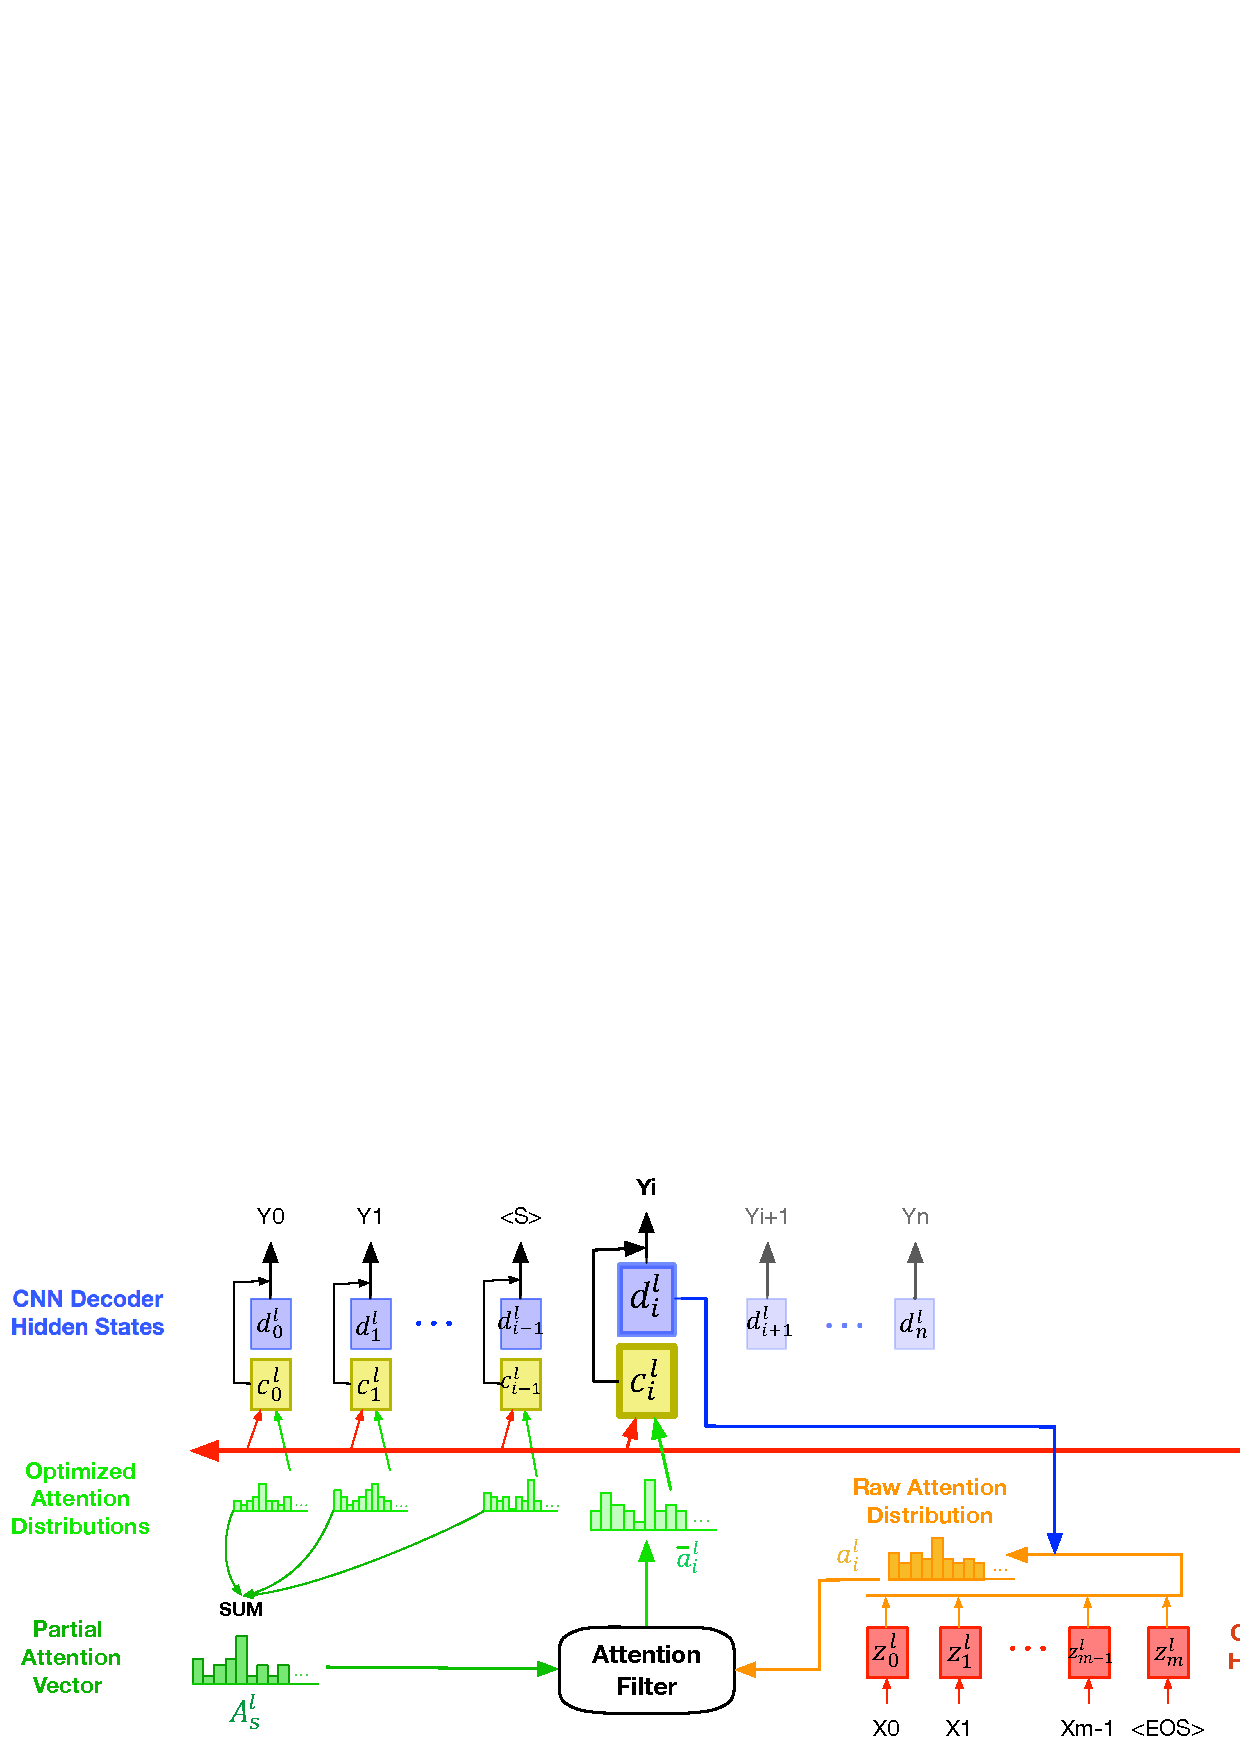
\includegraphics[width=0.9\linewidth]{./model.pdf}
	\caption{The architecture of MAI.}
	\label{fig:model}
\end{figure}
%We use the same methods to get
%noisy OAs embedding $\textbf{x}^p$=$(x^p_{0,0},x^p_{1,0},...,x^p_{u,U})$ 
%and noisy OSs embedding $\textbf{x}^s$=$(x^s_{0,0},x^s_{1,0},...,x^s_{v,V})$.
%We input noisy OAs to OA encoder and noisy ISs to IS encoder.
%$H^p_j$ and $H^s_{j'}$ is the encoder hidden state for $j$-th OA pair
%and $j'$-th IS sentence through LSTM layers.
%We take the last hidden state $H^p_U$ and $H^s_V$
%to represent opinion-aspect (generalized) information 
%and implicit sentences (specific) information.
We use $h^p_{i,j}$ and $h^s_{i',j'}$ to denote the encoder hidden state for $i$-th words in $j$-th OA pair
and $i'$-th word in $j'$-th IS sentence.
Inspired by~\citet{DialogMV2020},
we describe $j$-th OA pair in noisy OAs by 
the representation of $j$-th special token, $h^p_{0,j}$.
Then we aggregate the information of all pairs in noisy OAs through LSTM 
%~\cite{LSTM1997,DialogMV2020} 
as:
\begin{equation}
	H^p_j = LSTM(h^p_{0,j}, H^p_{j-1})
\end{equation}
%The last hidden state $H^p_U$.
where $H^p_j$ is the encoder hidden state for $j$-th OA.
We use the last hidden state $H^p_U$ as the OA representation.
Similary, we can get the IS representation $H^s_V$.
The {\em OA probability} $	\widetilde{\lambda}^p$ and 
{\em IS probability} $	\widetilde{\lambda}^s$ are calculated by:
\begin{equation}
	\widetilde{H}^p_U = \tanh(WH^p_U+b) 
\end{equation}
\begin{equation}
	\widetilde{H}^s_V = \tanh(W'H^s_V+b') 
\end{equation}
\begin{equation}
    \lambda^p = \frac{\exp(\widetilde{H}^p_U {^\top} v^p)}{\exp(\widetilde{H}^p_U {^\top} v^p)+\exp(\widetilde{H}^s_V {^\top} v^s)} 
\end{equation}

\begin{equation}
	\widetilde{\lambda}^p =\frac{ \lambda^{p\frac{1}{T}}}{\lambda^{p\frac{1}{T}}+(1-\lambda^p)^{\frac{1}{T}}}
	\label{eq:T}
\end{equation}
\begin{equation}
	\widetilde{\lambda}^s =1-\widetilde{\lambda}^p 
\end{equation}
where $v^p$ and $v^s$ respectively denote the randomly initialized context vector of OA encoder and IS encoder.
$W$ and $b$ are parameters. $T$ is the temperature for sharpening the attention distribution between encoders.
At each decoding step $t$, 
$C_t^p$ is the weighted sum of encoder hidden states of OA with Encoder-Decoder Attention (Enc-Dec Attn) as weight. 
$C_t^s$ is the weighted sum of IS encoder.
The combinational context vector $C_t$ for decoding is:
%of the Encoder-Decoder Attention 
%is the weighted sum of $C_t^p$ and $C_t^s$ as:
%is computed as:
%The combinational context vector $C_t$ for decoding is:
\begin{equation}
	C_t = \widetilde{\lambda}^p C_t^p +  \widetilde{\lambda}^s C_t^s
\end{equation}
$C_t$ should be modified by feed-forward network and becomes $G_t$. 
The probability distribution of generating $y_t$ is:
\begin{equation}
p(y_t|y_0,...,y_{t-1}, \textbf{x}^p,\textbf{x}^s)=softmax(WG_{t-1}+b)
\end{equation}
where $W$ and $b$ is the trainable parameters.
%In this model, the decoder hidden state of MAGOS is $\mathbf{Z}=(Z_0,...,Z_T)$. The decoder state at timestep $t+1$ should be calculated from
%$Z_t$ and $C_t$. 
%We also use the $softmax$ function to compute the probability distribution of 
%generation over $\mathbf{Z}$.
%The probability distribution over vocabulary of decoder is the same as Equation \ref{eq:decode}.

\subsubsection{Training MAI based on BAG (MB)}
%\subsubsection{MB}
%\textbf{Optimization: MAI based on BAG (MB)}
For optimization, we first train BAG to learn the explicit information from noisy OAs.
%Summaries generated by BAG
Then, we further fine-tune MAI based on the pretrained
BAG, enhancing the generated summary with
implicit opinion from noisy ISs.
%\KZ{Earlier you gave me the impression that BAG, AI and MAI etc, are all alternative
%summarization models that work on the synthetic pairs. But after this section,
%it seems that these models work together as components to a bigger thing?}

%We extract OAs and ISs of multi-review as noisy OAs and noisy ISs,
%which are the input of models.
%The human-written summaries are output.



